\section{On the reconstruction of W bosons}
\label{sec:Wreconstruction}
This section adresses the challenge of the reconstruction of the hadronically decaying \Wboson.
The \Wboson decays into exactly two quarks, but the
detector signature varies significantly depending on the event topology. 
While the two quarks typically form two distinct jets reconstructed via standard jet clustering, 
a third jet may arise from final-state radiation off one of the quarks. 
At high \Wboson momentum, the decay products become collimated due to Lorentz boosting and are merging into a single jet.
This leads to two main challenges: handling diverse jet multiplicities and resolving combinatorial ambiguities in the reconstruction.
The goal is to identify a robust reconstruction algorithm that can be applied on particle and reconstruction level
that effectively addresses these issues while remaining simple and practical to implement.

This study employs a subsample of the nominal PH+PY8 \ttbar simulation with the loose event selection described in the previous section.
Various jet-combinations are considered as possible candidates for the \Wboson.
A purity $p$ is defined as the number of matched events divided by all events passing the loose selection, where
matched events include all events where the angular distance $\Delta R$ between the true \Wboson before the decay into quarks \Wtruth
with the selected candidate reconstructed from jets \Wcand is smaller than 0.5:
\begin{equation}
	p = \frac{\#(\text{Events with}~ \Delta R(\Wtruth, \Wcand)<0.5)}{\#\text{Events}}.
    \label{eq:Wpurity}
\end{equation}
The candidate can be either the particle level or the reconstructed level candidate.
Given the large size of the analyzed data set, purity is prioritized over efficiency. 
A reduction in efficiency and consequently in the total event count is accepted in exchange for a cleaner, more reliable event selection.

Only light jets are considered for the reconstruction.
Several selection rules are tested with respect to the purity they can achieve:
\begin{itemize}
    \item Single jet [max(\pt(j))] selects highest-\pt jet in the event
    \item Dijet [max(\pt(j))] selects the hardest combination of two jets
    \item Dijet [min($|m_{jj}-m_W|$)] chooses the dijet combination whose invariant mass is closest to the true \Wboson mass
    \item Dijet [min($\Delta$ R(j,j) selects the dijet pair with the smallest angular separation
    \item Dijet [j$_1$+j$_2$] combines the four-vectors of the two leading light jets
\end{itemize}

The purity as a function of \(p_{T}(\Wtruth)\) for the \Wparticle and \Wreco reconstruction are displayed in Figure~\ref{fig:Whadreco:nocut} for the different selection criteria. The error band shows the statistical uncertainty of the MC sample.
\begin{figure}[ht!]
	\centering
	\begin{subfigure}[b]{0.49\linewidth}
		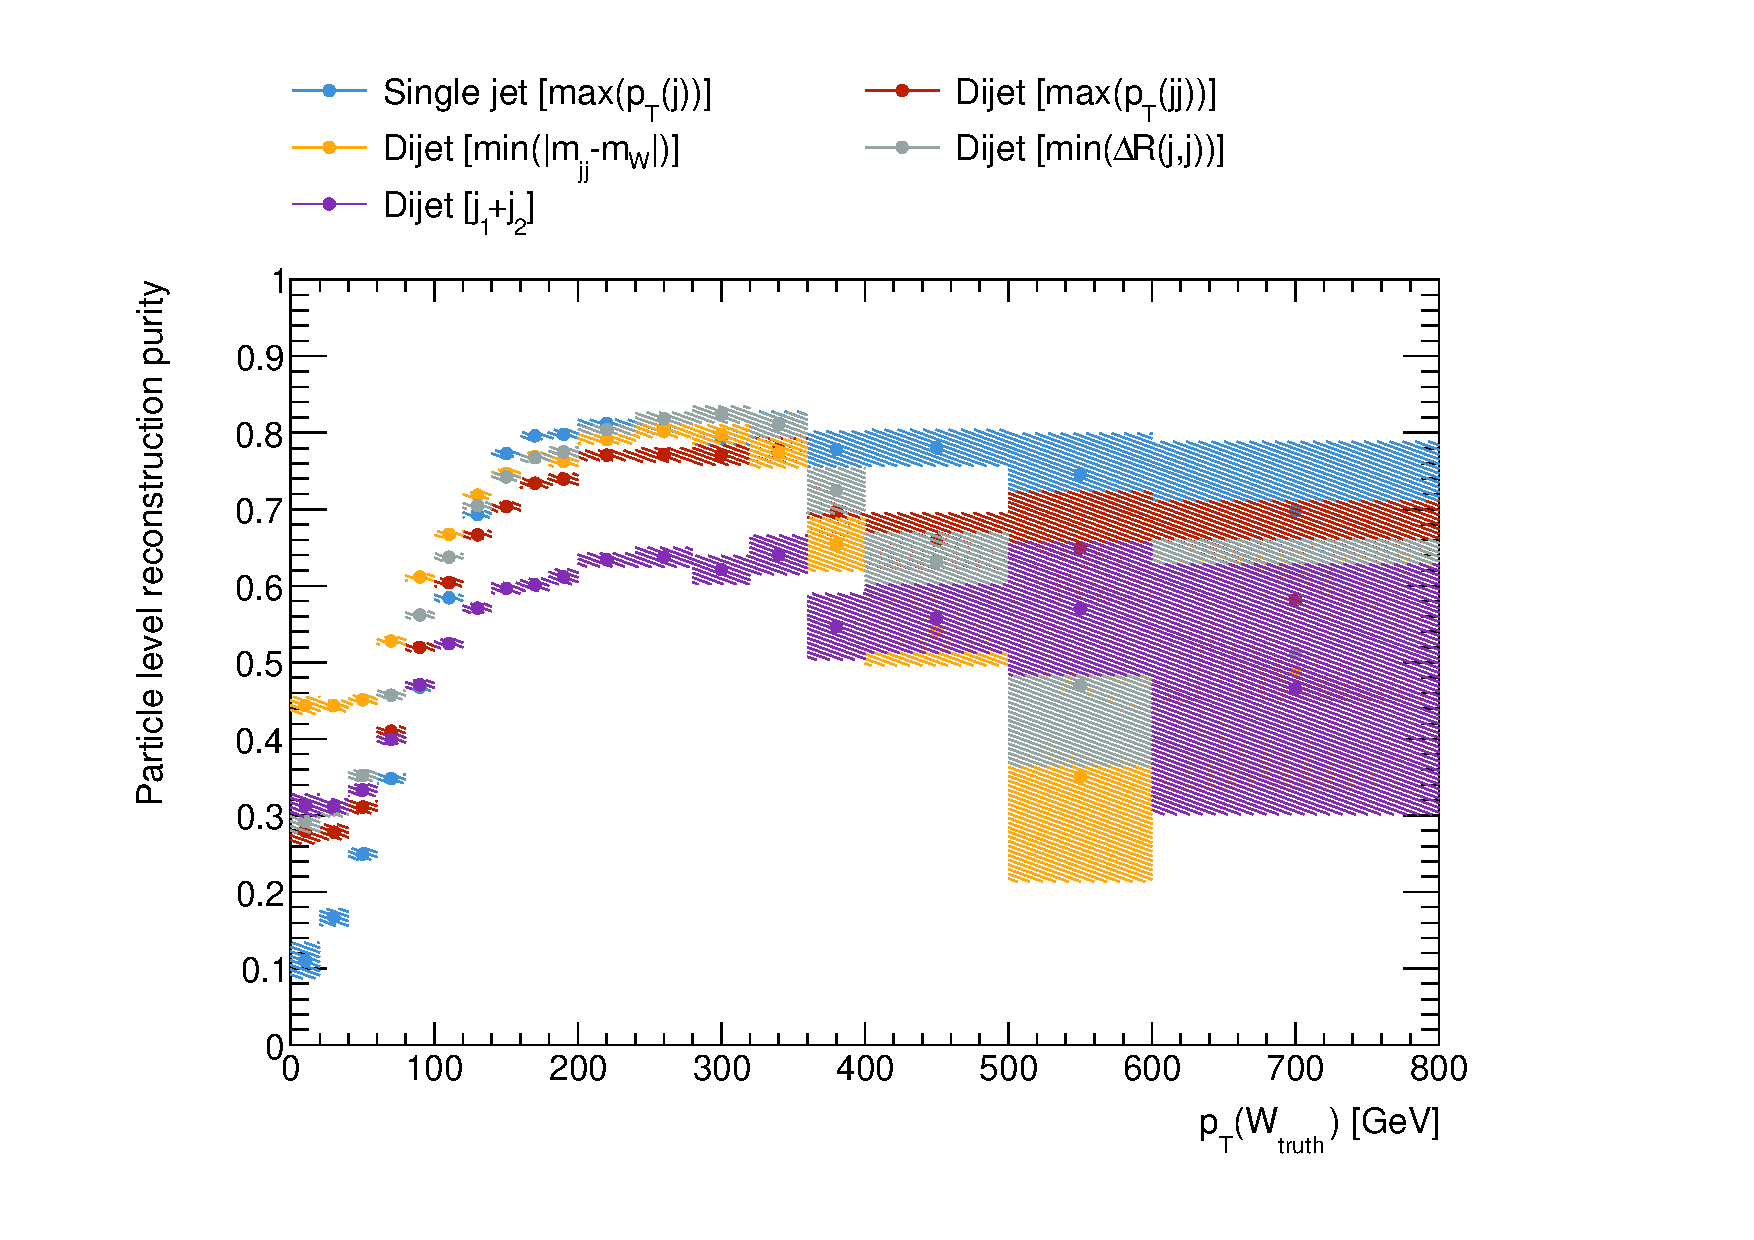
\includegraphics[width=1.\linewidth, page=1]{figures/WbWb/WhadReconstruction/purity.pdf}
		\caption{Purity for the particle level \Whad\\
        reconstruction.}
		\label{fig:Whadreco:partnocut}
	\end{subfigure}
	\begin{subfigure}[b]{0.49\linewidth}
		\includegraphics[width=1.\linewidth, page=2]{figures/WbWb/WhadReconstruction/purity.pdf}
		\caption{Purity for the detector level \Whad \\
        reconstruction.}
		\label{fig:Whadreco:reconocut}
	\end{subfigure}
	\caption{Comparison of the particle and detector level reconstruction of the hadronically decaying \Wboson from light jets.
    The various candidates are explained in the text and the purity is defined in Eq.~\eqref{eq:Wpurity}.}
	\label{fig:Whadreco:nocut}
\end{figure}
The highest purities in the low \pT regime \(\pT < 100 \GeV\) are obtained 
by selecting the dijet combination whose mass is closest to the true \Wboson mass (orange).
The performance in the medium \pT range is similar for all considered options with a purity around \(80\%\).
Only the purple curve selecting the four-vector sum of the leading and sub-leading light jet
performs slightly poorer with a purity of around \(60\%\).
At high \Wboson momenta, a preference towards high-momenta candidates can be observed: The leading light jet (light blue) as well as the hardest dijet combination (red) perform best.
The purities obtained for the particle and detector level studies are similar, with slightly higher values obtained for the particle level.

\begin{figure}[ht!]
	\centering
	\begin{subfigure}[b]{0.49\linewidth}
		\includegraphics[width=1.\linewidth, page=3]{figures/WbWb/WhadReconstruction/purity.pdf}
		\caption{Purity for the particle level \Whad \\ reconstruction.}
		\label{fig:Whadreco:partmasscut}
	\end{subfigure}
	\begin{subfigure}[b]{0.49\linewidth}
		\includegraphics[width=1.\linewidth, page=4]{figures/WbWb/WhadReconstruction/purity.pdf}
		\caption{Purity for the detector level \Whad \\ reconstruction.}
		\label{fig:Whadreco:recomasscut}
	\end{subfigure}
	\caption{Comparison of the particle and detector level reconstruction of the hadronically decaying \Wboson from light jets. 
        The various candidates are explained in the text and the purity is defined in Eq.~\eqref{eq:Wpurity}.
		Only events passing $60<m(\Wcand)<100$ GeV are considered for the calculation of the purity.}
	\label{fig:Whadreco:masscut}
\end{figure}

The study is repeated with the addition of a selection cut on the mass of the \Wboson candidate \(60<m(\Wcand)<100\GeV\). This cut is applied in the nominator as well as the denominator of the purity definition.
Single bins are merged in the plotting step to reduce the statistical uncertainties.
The results are shown in Figure~\ref{fig:Whadreco:masscut}. 
Selecting the jet combination whose invariant mass is closest to the true \Wboson mass (orange curve) achieves $15\%$ lower purities compared
to the other options.
The highest purity is obtained by selecting the dijet system containing leading and sub-leading light jet (purple).
At highest \Wboson momenta, selecting the leading jet results in the highest purity.
The statistical uncertainties in that region are significantly smaller, compared to the other options.

\begin{figure}[ht!]
	\centering
	\begin{subfigure}[b]{0.49\linewidth}
		\includegraphics[width=1.\linewidth, page=5]{figures/WbWb/WhadReconstruction/purity.pdf}
		\caption{Purity for the particle level \Whad \\ reconstruction.}
		\label{fig:Whadreco:combinedpart}
	\end{subfigure}
	\begin{subfigure}[b]{0.49\linewidth}
		\includegraphics[width=1.\linewidth, page=6]{figures/WbWb/WhadReconstruction/purity.pdf}
		\caption{Purity for the detector level \Whad \\ reconstruction.}
		\label{fig:Whadreco:combinedreco}
	\end{subfigure}
    \\
    \begin{subfigure}[b]{0.49\linewidth}
		\includegraphics[width=1.\linewidth, page=7]{figures/WbWb/WhadReconstruction/purity.pdf}
		\caption{Purity for the particle level \Whad \\ reconstruction with mass cut.}
		\label{fig:Whadreco:combinedpartmasscut}
	\end{subfigure}
	\begin{subfigure}[b]{0.49\linewidth}
		\includegraphics[width=1.\linewidth, page=8]{figures/WbWb/WhadReconstruction/purity.pdf}
		\caption{Purity for the detector level \Whad \\ reconstruction with mass cut.}
		\label{fig:Whadreco:combinedrecomasscut}
	\end{subfigure}
	\caption{Comparison of the particle (left) and detector level (right) reconstruction of the hadronically decaying \Wboson from light jets. 
        Different combinations of jets are pre-selected as the \Wboson candidate. The candidate that minimizes \(|m(\Wboson)-m(\Wcand)|\) is selected as pseudo-\Wboson.
        Only events passing the $60<m(\Wcand)<100$ GeV cut are considered in the lower row.
        The results are compared to the purities obtained from a DNN. More information is given in the text.}
	\label{fig:Whadreco:combined}
\end{figure}

It becomes evident, that one should preselect different jet combinations as preliminary candidates to account for the different topologies from resolved and boosted events.
Two combinations are compared in Figure~\ref{fig:Whadreco:combined}.
The blue curve labelled "1-,2-,3-jet" preselects a total of five objects: the leading jet, the sub-leading jet, the four-vector sum of the two, the leading dijet and the leading three-jet combination. The "1-,2-jet" algorithm displayed in red drops the last two candidates from the list.
Both options produce high purities, but the best result is obtained with the latter algorithm.

The "1-,2-jet" algorithm was chosen as the final algorithm for the analysis event selection and observable definitions.
The purity exceeds $90\%$ for \Wboson momenta larger than 120\GeV.
A pseudo-\Wboson can be found for each event.
Selection cuts can be applied on \Wcand. The mass cut $60<m(\Wcand)<100$ GeV is motivated by the purity studies.
An additional cut on \pT(\Whad) will be applied to ensure a good quality of the reconstruction for each event.
A \(\pT > 80\GeV\) cut-off was chosen to ensure, that the purity exceeds \(60\%\) for the particle and detector level reconstruction.

\begin{figure}[ht!]
	\centering
	\begin{subfigure}[b]{0.49\linewidth}
		\includegraphics[trim={2cm 0cm 5cm 0cm}, clip, width=1.\linewidth, page=25]{figures/WbWb/WhadReconstruction/purity.pdf}
		\caption{Mass distribution of the detector level \Whad candidate.}
		\label{fig:Whadreco:partmass}
	\end{subfigure}
	\begin{subfigure}[b]{0.49\linewidth}
		\includegraphics[trim={2cm 0cm 5cm 0cm}, clip, width=1.\linewidth, page=24]{figures/WbWb/WhadReconstruction/purity.pdf}
		\caption{Mass distribution of the detector level \Whad candidate.}
		\label{fig:Whadreco:recomass}
	\end{subfigure}
	\caption{Comparison of the particle and detector level mass distributions.}
	\label{fig:Whadreco:masscut}
\end{figure}

The results obtained from the combinatorics-based reconstruction approach are compared to a Machine-Learning-based reconstruction.
A fully-connected classification neural network is designed and trained for that purpose.
The network consists of five layers with 8, 16, 32, 16, 8 nodes, respectively.
This results in a total of 1401 trainable parameters.

The five hardest light jets are used and
every 1-, 2- and 3-jet combination built from the input jets is considered as a \Wboson candidate.
This results in a total of $5+10+10=25$ combinations.
The four-vectors of the jet combinations are passed as input to the network.
The jet combination with the smallest distance to \Wtruth in \(\Delta R\) is labeled with "1", while "0" is assigned to all other combinations as training label.

The study is performed on the same \ttbar subsamples used earlier.
The data is split equally into training and validation samples and the purities are calculated on the validation sample.
The statistical uncertainties are thus not comparable to the ones obtained in the classical method.